Resultater:

LC-kredsløb (Kapacitor):

For LC-kredsløbet blev der foretaget målinger for spændingen over kapacitoren ved forskellige frekvenser. Første måling er foretaget ved $1 kHz$, hvorefter de følgende målinger er foretaget med et $0,5 kHz$ interval op til sidste måling ved $5,5 kHz$. Resultaterne er indsat i nedenstående graf. Skema X angiver resultaterne for spændingen i forhold til den givne frekvens.

\begin{figure}[H]
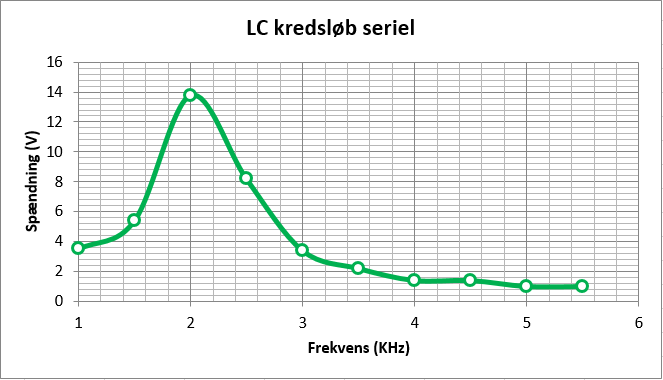
\includegraphics[scale=1]{Graf3}
\end{figure}

\begin{tabular}{|r|r|r|r|r|r|r|r|r|r|r|} \hline
kHz & 1 & 1,5 & 2 & 2,5 & 3 & 3,5 & 4 & 4,5 & 5 & 5,5 \\ \hline
V & 3,5 & 5,4 & 13,8 & 8,2 & 3,4 & 2,2 & 1,4 & 1,4 & 1 & 1 \\ \hline
\end{tabular}

Graf X viser sammenhængen mellem spændingen og frekvensen over kapacitoren, når frekvensen øges. Ved en frekvens på $1 kHz$ er spændingen over kapacitoren $3,5 V$. Ved en frekvens på $1,5 kHz$ er spændingen øget til $5,4 V$, hvorefter der sker en markant stigning til en spænding på $13,8 V$ ved en frekvens på $2 kHz$. Fra frekvensen på $2 kHz$ og til en frekvens på $4 kHz$ er spændingen over kapacitoren faldet til $1,4 V$, hvorefter funktionen flader ud, og spændingen næsten holdes stabil til en frekvens på $5,5 kHz$.

LCR-kredsløb (Resistor):

Første sæt målinger for LCR-kredsløbet angiver spændingen over resistoren ved en stigende frekvens. Målingerne er foretaget fra $1 kHz$ til $10 kHz$ med et interval på $1 kHz$ for hver måling. Resultaterne for målingerne er plottet i nedenstående graf. Skema X angiver resultaterne for spændingen i forhold til den givne frekvens.

\begin{figure}[H]
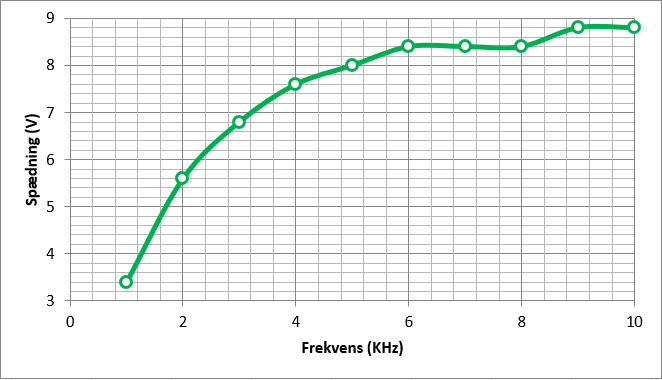
\includegraphics[scale=1]{Graf7}
\end{figure}

\begin{tabular}{|r|r|r|r|r|r|r|r|r|r|r|} \hline
kHz & 1 & 2 & 3 & 4 & 5 & 6 & 7 & 8 & 9 & 10 \\ \hline
V & 3,4 & 5,6 & 6,8 & 7,6 & 8 & 8,4 & 8,4 & 8,4 & 8,8 & 8,8 \\ \hline
\end{tabular}

Graf X viser, hvordan spændingen over resistoren er lav ved en frekvens på $1 kHz$. Ved en stigning i frekvens viser det sig, at spændingen stiger som en eksponentielt aftagende funktion. Fra en frekvens på $1 kHz$ til $4 kHz$ stiger spændingen over modstanden fra $3,4 V$ til $7,6 V$, men ved de efterfølgende stigninger i frekvens flader funktionen ud, og der sker kun en spændingsstigning på $0,4 V$ fra en frekvens på $6 kHz$ til $10 kHz$.

LCR-kredsløb (Spole):

De næste målinger der er foretaget på LCR-kredsløbet viser sammenhængen mellem spændingen og frekvensen for induktoren. Her foretages målingerne igen ved en frekvens fra $1 kHz$ til $10 kHz$ med et stigende interval på $1 kHz$. Nedenstående graf viser resultaterne for førsøget, hvor skema X angiver resultaterne for spændingen i forhold til den givne frekvens.

\begin{figure}[H]
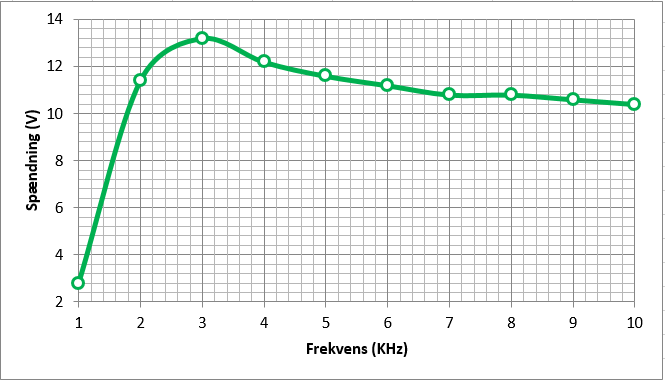
\includegraphics[scale=1]{Graf6}
\end{figure}

\begin{tabular}{|r|r|r|r|r|r|r|r|r|r|r|} \hline
kHz & 1 & 2 & 3 & 4 & 5 & 6 & 7 & 8 & 9 & 10 \\ \hline
V & 2,8 & 11,4 & 13,2 & 12,2 & 11,6 & 11,2 & 10,8 & 10,8 & 10,6 & 10,4 \\ \hline
\end{tabular}

Spændingen over induktoren stiger fra $2,8 V$ ved en frekvens på $1 kHz$ til $11,4 V$ ved en frekvens på $2 kHz$. Spændingen stiger fortsat til $13,2 V$ ved en frekvens på $3 kHz$, hvorefter spændingen over induktoren begynder at falder ved en højere frekvens. Faldet i spændingen sker kun gradvist og ved en frekvens på $7 kHz$, er funktionen næsten ved en stabil spænding.